\subsection{Deep Models on Structured Data}
\label{sec:deep1}

\outline{Explain next step in model evolution}
Linear models directly map from inputs to predictions.
Assuming the inputs stay the same, the next step in neural network evolution
should be to add hidden layers.
The reasoning behind this is the increased capability of the model to learn intermediate
feature representations, which in turn should enable more accurate predictions.
This section examines application of deep feedforward networks to the problem
of engagement prediction.
Model architectures are introduced in Chapter~\ref{sub:deep1_architecture}
\outline{Introduce subsection structure}, before the training process is detailled
in Chapter~\ref{sub:deep1_training}.
Finally, results and accompanying analysis are presented in Chapter~\ref{sub:deep1_performance}.

\subsubsection{Model architecture}
\label{sub:deep1_architecture}

\outline{Starting point: same inputs and outputs as before, but adding hidden
(feedforward) layers inbetween}
\outline{Why feedforward? Only reasonably applicable layer type since input features
are temporarily and locally unrelated}
\outline{Question: how many hidden layers to add? No strict rules exist, only heuristics.}
\addcitation{Link to heuristics article}
\outline{Answer: testing different architectures for model selection; trade-off between performance and training time}

\begin{table}
\begin{tabular}{llrr}
\toprule
Hidden layers & Hidden units & Classification loss & Regression loss \\
\midrule
2 & 16 & 0.8203 & 2,593.2 \\
2 & 32 & 0.7502 & 2,520.2 \\
2 & 64 & 0.7346 & 2,509.9 \\
3 & 16 & 0.7888 & 2,529.9 \\
3 & 32 & 0.7430 & 2,557.3 \\
3 & 64 & 0.7160 & 2,465.1 \\
4 & 16 & 0.7792 & 2,588.5 \\
4 & 32 & 0.7261 & 2,477.5 \\
4 & 64 & \textbf{0.7088} & 2,435.8 \\
5 & 64 & 0.7128 & \textbf{2,386.1} \\
6 & 64 & 0.7016 & 2,410.1 \\
\bottomrule
\end{tabular}
\caption{Summary of model selection results}
\label{tab:dm1_selection_results}
\end{table}

\outline{Selection process: celebrity data set, 50 (classification) resp. 100
(regression) iterations with same settings as before}
\outline{Hidden layer variants: 2-6, hidden unit variants: 16, 32, 64}
\outline{Results: 4 layers w/ 64 units for classification, 5 layers w/ 64 units 
for regression}
\outline{Adding units yields better results than adding layers}
\outline{Adding more layers only leads to minor improvement and more unstable
training process (i.e., overfitting)}

\begin{figure}[h]
\begin{subfigure}{.4\textwidth}
  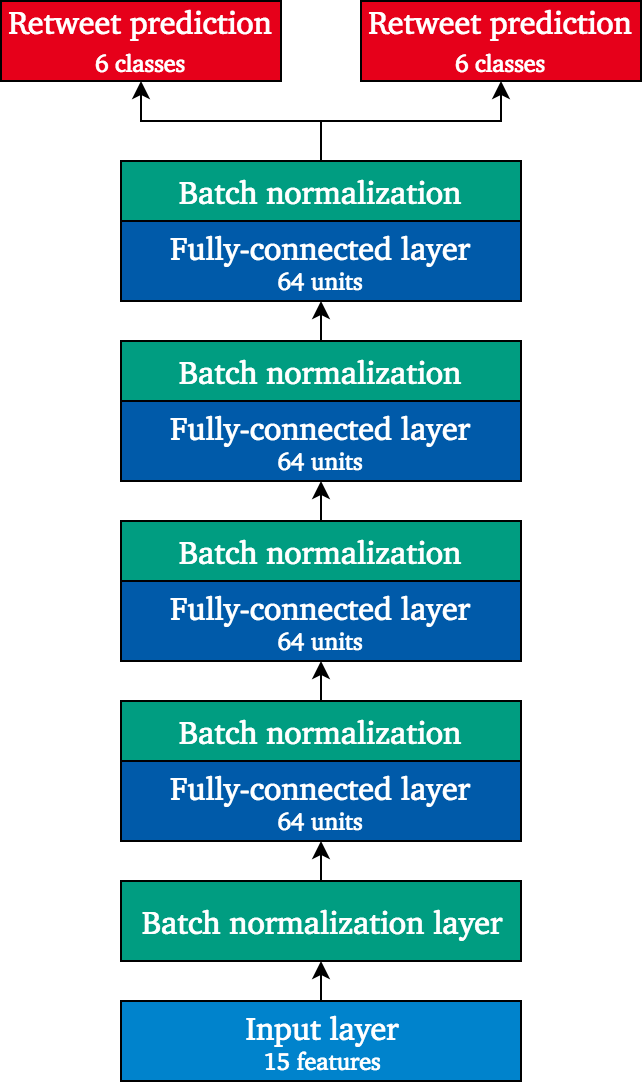
\includegraphics[width=.95\linewidth]{img/deep_1_class_architecture}
  \caption{Classification model}
  \label{fig:deep1_architecture_1}
\end{subfigure}%
\begin{subfigure}{.4\textwidth}
  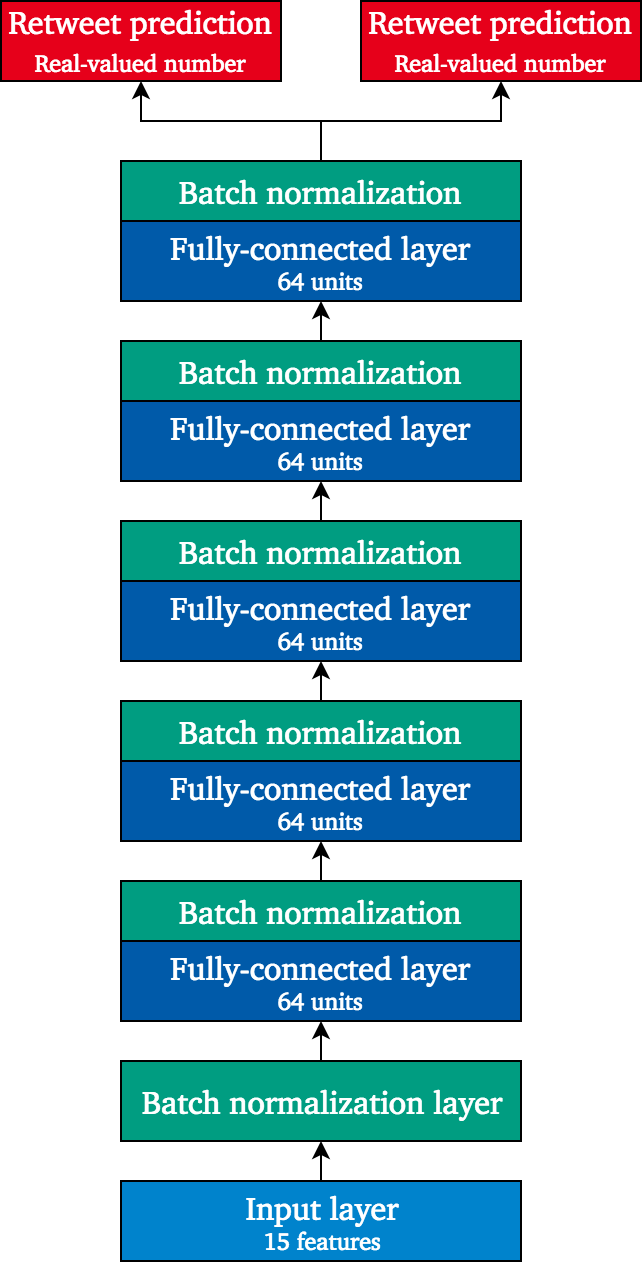
\includegraphics[width=.95\linewidth]{img/deep_1_regr_architecture}
  \caption{Regression model}
  \label{fig:deep1_architecture_2}
\end{subfigure}
\caption{Architecture of deep feedforward network}
\label{fig:deep1_architecture}
\end{figure}

\outline{BatchNormalization after each layer to speed up training process and
avoid overfitting}

\subsubsection{Training process}
\label{sub:deep1_training}

\outline{Setting is mostly unchanged: same training/validation split, optimizer
and cost functions}
\outline{Only change: regression model trained for only 100 iterations since they
converge faster}

\subsubsection{Model performance}
\label{sub:deep1_performance}

\begin{table}
  \begin{tabular}{lrrrrrrr}
    \toprule
    & \multicolumn{4}{l}{Classification} & \multicolumn{3}{l}{Regression} \\
    \midrule
    Data set & CCE & Acc & Ret Acc & Fav Acc & MAE & Ret MAE & Fav MAE \\
    \midrule
    Celebrities & 0.71 & 70.29\% & 66.30\% & 74.28\% & 2,345.85 & 1,165.19 & 3,526.51 \\
    Politicians & 0.81 & 64.75\% & 63.37\% & 66.12\% & 424.05 & 247.40 & 600.69 \\
    Companies & 0.72 & 70.07\% & 72.38\% & 67.76\% & 19.72 & 10.92 & 28.52 \\
    Combined & 1.03 & 55.50\% & 57.75\% & 53.25\% & 549.93 & 210.71 & 889.16 \\
    \bottomrule
  \end{tabular}
  \caption{Summary of results for deep feedforward network}
  \label{tab:deep1_results}
\end{table}

\outline{Overall performance increases (cost function lower for both tasks
across all data sets)}
\outline{Additional information: models start to overfit slightly (esp. company
classification => training loss is 0.64)}
\outline{Classification accuracy improvements between 10 and 20 \% (celebrity performance
improvements are strongest), 65 to 70\% of validation examples are classified correctly}
\outline{Improvements are slightly higher for favorite classification (except for politicians)}
\outline{Relation between RetAcc and FavAcc unchanged}
\outline{Interesting: classification works best for celebrity data (previously worst performance)}
\outline{MAE results lowered by 12 (politicians) to 33\% (celebrities)}
\outline{Improvements mostly driven by strong decreases in FavMAE (decreases
higher across the board)}
\outline{More details on classification and regression performance in the following}

\begin{figure}[h]
\begin{subfigure}{.5\textwidth}
  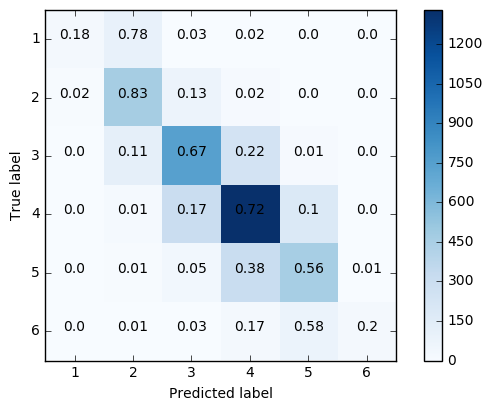
\includegraphics[width=.95\linewidth]{img/celeb_d1_cm_retweets}
  \caption{Celebrity data set}
  \label{fig:retw_distr_sub1}
\end{subfigure}%
\begin{subfigure}{.5\textwidth}
  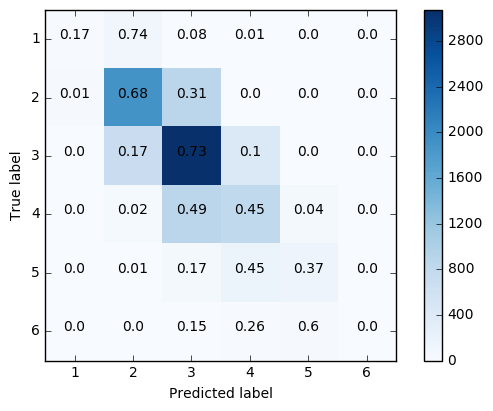
\includegraphics[width=.95\linewidth]{img/polit_d1_cm_retweets}
  \caption{Politician data set}
  \label{fig:retw_distr_sub2}
\end{subfigure}
\begin{subfigure}{.5\textwidth}
  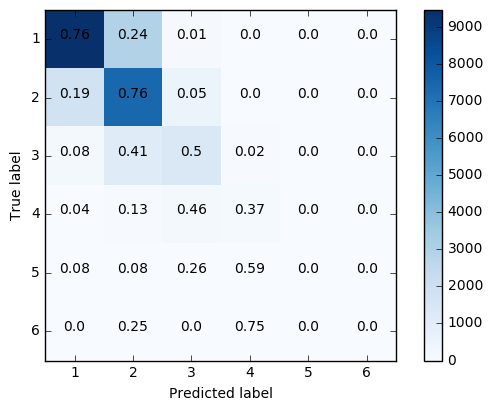
\includegraphics[width=.95\linewidth]{img/corp_d1_cm_retweets}
  \caption{Company data set}
  \label{fig:retw_distr_sub3}
\end{subfigure}%
\begin{subfigure}{.5\textwidth}
  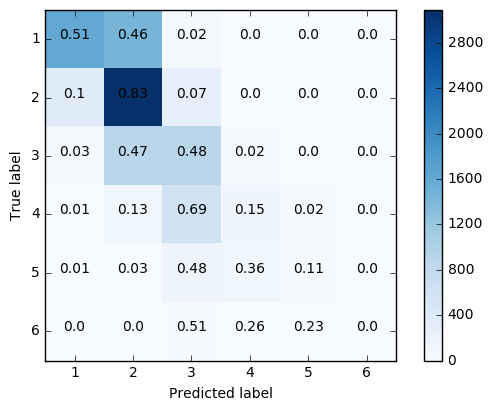
\includegraphics[width=.95\linewidth]{img/comb_d1_cm_retweets}
  \caption{Combined data set}
  \label{fig:retw_distr_sub4}
\end{subfigure}%
\caption{Confusion matrices for deep feedforward classification models}
\label{fig:d1_cm}
\end{figure}

\outline{More correctly classified examples (see main diagonal)}
\outline{Celebrities: Classes around median are predicted more accurately than border classes}
\outline{Celebrities: Not biased towards biggest class, misclassifications are `better'}
\outline{Sames is true for politicians}
\outline{Companies: model is good at predicting first two classes}
\outline{Companies: better (but not good) performance on classes 3 and 4}
\outline{Companies: classes 5 and 6 are still never predicted}

\begin{table}
  \begin{tabular}{lrrrrrrr}
    \toprule
    & \multicolumn{7}{c}{Actual retweets} \\
    \midrule
    Data set & 0 & 1-10 & 10-100 & 100-1k & 1-10k & 10-100k & >100k \\
    \midrule
    Celebrities & - & 51.9 & 161.4 & 701.3 & 3,884.9 & 21,557.9 & - \\
    Politicians & 46.0 & 109.7 & 184.5 & 781.0 & 3,973.1 & - & - \\
    Companies & 1.5 & 5.9 & 49.5 & 605.7 & - & - & - \\
    Combined & 0.4 & 5.2 & 32.0 & 233.6 & 2,088.3 & 21,919.0 & 86,217.9 \\
    \bottomrule
    \toprule
    & \multicolumn{7}{c}{Actual favorites} \\
    \midrule
    Data set & 0 & 1-10 & 10-100 & 100-1k & 1-10k & 10-100k & >100k \\
    \midrule
    Celebrities & - & 7.4 & 268.5 & 638.1 & 3,139.2 & 19,212.0 & 45,031.3 \\
    Politicians & 92.6 & 130.4 & 234.1 & 864.5 & 3,528.9 & 12,167.6 & - \\
    Companies & 6.5 & 6.6 & 39.7 & 743.1 & 1,314.0 & - & - \\
    Combined & 0.4 & 4.4 & 32.1 & 355.8 & 3,279.5 & 26,871.1 & 169,920.5 \\
    \bottomrule
  \end{tabular}
  \caption{Mean absolute errors for specific ranges of actual engagement}
  \label{tab:d1_regression_eval}
\end{table}

\outline{Using MAE requires mean calculation => need for more detailed performance
evaluation}
\outline{Errors need to be considered in relation to magnitude of actual counts}
\outline{Table shows MAE for specific ranges of actual engagement counts}
\outline{Dash denotes absence of validation data for this range}
\outline{Observation: MAE increases with rising engagement counts}
\outline{Order of magnitudes vary drastically (can be expected)}

